% \documentclass{report}
% \usepackage[utf8]{inputenc}
% \usepackage[brazil]{babel}

\documentclass[oneside,a4paper,12pt]{normas-utf-tex}

\usepackage{breakurl}
\usepackage[alf,abnt-emphasize=bf,bibjustif,recuo=0cm, abnt-etal-cite=2]{abntcite}
\usepackage[brazil]{babel}
\usepackage[utf8]{inputenc}
\usepackage{amsmath}
\usepackage{graphicx,subfig}
\usepackage{times}
\usepackage[plain]{fancyref}
\usepackage{float}
\usepackage{pdfpages}
\usepackage{enumitem}
\usepackage{longtable}

%%% Complemento para tabelas
\usepackage{booktabs, multirow}
\setlength{\heavyrulewidth}{0.1em}
\renewcommand{\toprule}{\midrule[\heavyrulewidth]}
\renewcommand{\arraystretch}{1.2}
%%%

\instituicao{Universidade Tecnológica Federal do Paraná}
\departamento{Departamento Acadêmico de Eletrônica}
\departamentodois{Departamento Acadêmico de Informática}
\programa{Curso de Engenharia de Computação}
\unidade{Oficina de Integração 3}

\titulo{\MakeUppercase{Mapeamento de ambientes com o robô Bellator}}
\documento{Primeiro entregável}

\autor{Luis Guilherme Machado Camargo}
\autordois{Pedro Alberto de Borba}
\autortres{Ricardo Farah}
\autorquatro{Stefan Campana Fuchs}
\autorcinco{Telmo Friesen}

\cita{CAMARGO, L.G.M; BORBA, P.A.; FARAH, R.; FUCHS, S.C.; FRIESEN, T}

\comentario{\UTFPRdocumentodata\ apresentada à Unidade Curricular de \UTFPRunidadedata\ do \UTFPRprogramadata\ da \ABNTinstituicaodata\ como requisito parcial para aprovação.}

\local{Curitiba}
\data{\the\year}

\begin{document}

\capa
\folhaderosto
\sumario
\chapter{Primeiro entregável 1 - 13/03/2013}

Conforme estabelecido na relação de deliverables do documento de análise tecnológica, este primeiro entregável consiste nos seguintes itens:
\begin{enumerate}[topsep=0pt, partopsep=0pt, itemsep=0pt]
	\item Versões iniciais dos diagramas de casos de uso e de classes (estação base).
	\item Versão inicial do diagrama em blocos (hardware).
	\item Explicação inicial de cada bloco (hardware).
\end{enumerate}


\chapter{Modelagem UML}

\section{Requisitos funcionais}

\begin{enumerate}[topsep=0pt, partopsep=0pt, itemsep=0pt]
%  \item A estação base deve receber informações de posicionamento do robô, processá-las e armazená-las na memória. Representado pelo requisito funcional: \textbf{``Estação base mostra na interface gráfica a posição do robô - RF\arabic{enumi}"}
%  \item A estação base deve receber informações de obstáculos detectados, processá-las e armazená-las na memória. Representado pelo requisito funcional: \textbf{"Estação base mostra na interface gráfica os novos obstáculos detectados pelo robô - RF\arabic{enumi}"}
  \item A estação base deve mostrar na interface gráfica um mapa 2D (atualizado automaticamente) representando o robô e os obstáculos detectados por ele. Representado pelo requisito funcional: \textbf{``Estação base mostra mapa 2D do robô e dos obstáculos detectados -- RF\arabic{enumi}''}.
  \item O usuátio pode salvar o mapa 2D no disco rígido. Representado pelo requisito funcional: \textbf{``O usuário pode salvar o mapa -- RF\arabic{enumi}''}.
  \item O usuário pode carregar o mapa 2D do disco rígido. Representado pelo requisito funcional: \textbf{``O usuário pode carregar o mapa -- RF\arabic{enumi}''}.
  \item A estação base deve mostrar na interface gráfica a imagem captada pela \textit{webcam} do robô. Representado pelo requisito funcional: \textbf{``Estação base mostra a imagem captada pela webcam -- RF\arabic{enumi}''}.
  \item O usuário pode movimentar o robô, controlando a velocidade de suas rodas remotamente pelo teclado da estação base. Representado pelo requisito funcional: \textbf{``O usuário pode movimentar o robô -- RF\arabic{enumi}''}.
  \item A estação base deve ser capaz de estabelecer conexão com o robô, informando o usuário caso a conexão ocorra com sucesso ou não. Representado pelo requisito funcional \textbf{``O usuário pode estabelecer a conexão entre o robô e a estação base -- RF\arabic{enumi}''}.
\end{enumerate}

\section{Requisitos não funcionais}

\begin{enumerate}[topsep=0pt, partopsep=0pt, itemsep=0pt]
  \item A imagem transmitida pela câmera do robô deve ser colorida. Representado pelo requisito não funcional: \textbf{``O robô deve enviar vídeo em imagem colorida para a estação base - RNF\arabic{enumi}''}.
  \item O robô deve transmitir as imagens de sua câmera em tempo real. Representado pelo requisito não funcional: \textbf{``O robô deve transmitir os dados de vídeo captados pela câmera em tempo real - RNF\arabic{enumi}''}.
%  \item O método de entrada do usuário deve se dar por meio de interface gráfica com o auxílio do mouse. Representado pelo requisito não funcional: \textbf{"O usuário pode interagir com o robô por meio do mouse - RNF0\arabic{enumi}"}.
%  \item O método de entrada do usuário deve se dar por meio de interface gráfica com o auxílio do teclado. Representado pelo requisito não funcional: \textbf{"O usuário pode interagir com o robô por meio do teclado - RNF0\arabic{enumi}"}.
\end{enumerate}


\section{Casos de uso identificados}

\begin{enumerate}[topsep=0pt, partopsep=0pt, itemsep=0pt]
  \item Visualização de mapa 2D na interface gráfica segundo os dados lidos dos sensores do robô. Representado pelo caso de uso: \textbf{``Mostrar mapa - UC\arabic{enumi}''}.
  \item Gravação do mapa em um arquivo no disco rígido. Representado pelo caso de uso: \textbf{``Salvar mapa - UC\arabic{enumi}''}. 
  \item Leitura do mapa de um arquivo do disco rígido. Representado pelo caso de uso: \textbf{``Carregar mapa - UC\arabic{enumi}''}.
  \item Leitura de informações dos sensores do robô. Representado pelo caso de uso: \textbf{``Ler amostras dos sensores - UC\arabic{enumi}''}.
  \item Visualização de imagens da \textit{webcam} do robô. Representado pelo caso de uso: \textbf{``Visualizar imagens da câmera - UC\arabic{enumi}''}.
  \item Alteração pelo usuário da velocidade das rodas do robô. Representado pelo caso de uso: \textbf{``Alterar velocidade das rodas - UC\arabic{enumi}''}.
  \item Solicitação de estabelecimento de conexão com o robô. \textbf{``Estabelecer conexão - UC\arabic{enumi}''}.
%  \item Inclusão de novos obstáculos e suas posições lidos do robô. Representado pelo caso de uso: \textbf{``Mostrar posição dos novos obstáculos detectados na tela - UC\arabic{enumi}''}.
  \item Consulta à documentação do robô pelo usuário. Representado pelo caso de uso: \textbf{``Consultar documentação do robô - UC\arabic{enumi}''}.
\end{enumerate}

Foram produzidos três Diagramas de Casos de Uso (Figuras \ref{fig:diagrama_caso_uso_estacao_base}, \ref{fig:diagrama_caso_uso_linux_embarcado} e \ref{fig:diagrama_caso_uso_placa_embarcada}) com base nos casos de uso apresentados. O primeiro diagrama representa o \textit{software} da estação base, e o segundo e o terceiro representam o sistema embarcado (TS-7260 e placa de baixo nível, respectivamente).

\begin{figure}[H]
  \centering
  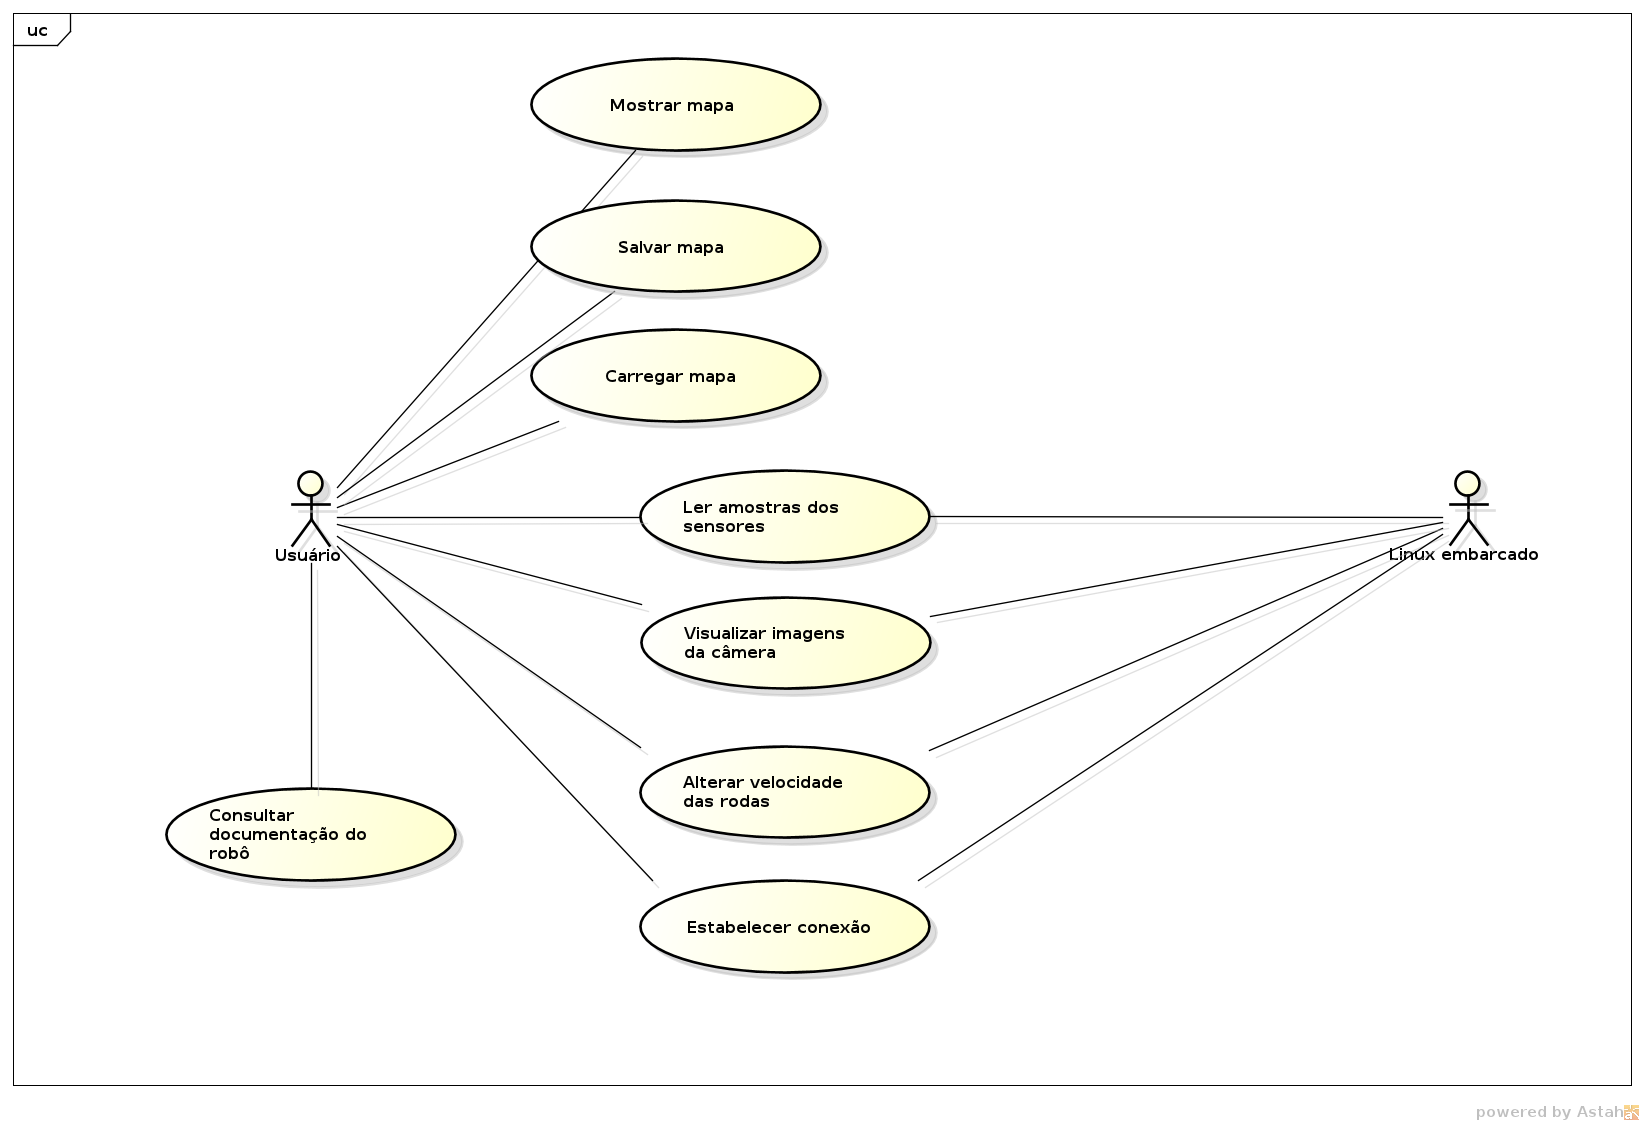
\includegraphics[width=\textwidth, keepaspectratio]{./figuras/diagrama_caso_uso_estacao_base.png}
  \caption{Diagrama de casos de uso do \textit{software} da estação base.}
  \label{fig:diagrama_caso_uso_estacao_base}
\end{figure}

\begin{figure}[H]
  \centering
  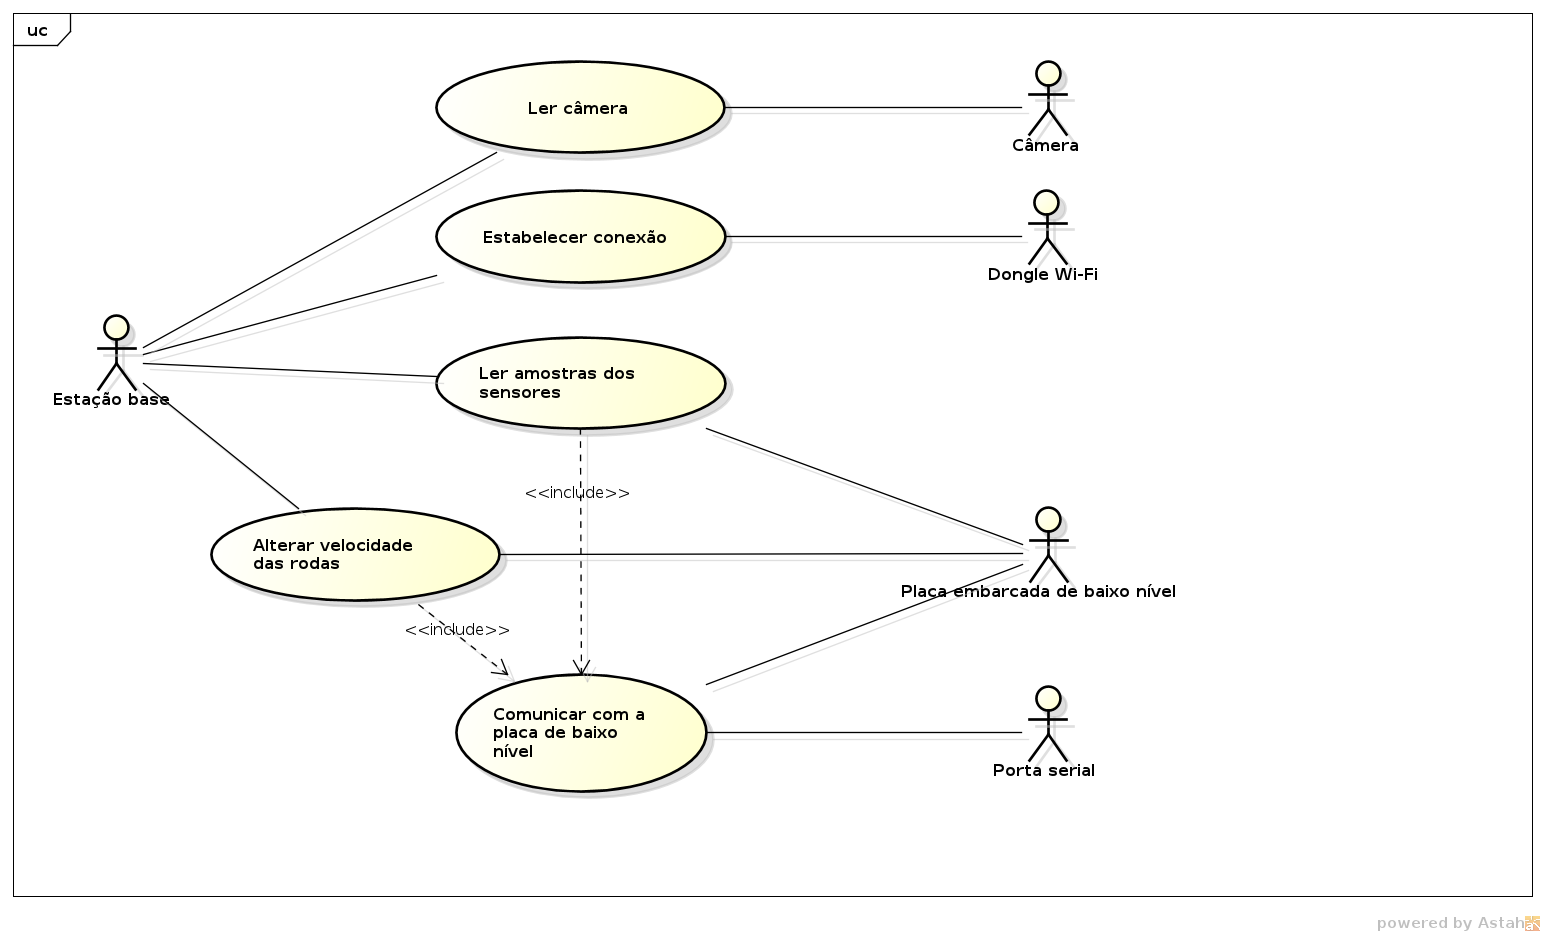
\includegraphics[width=\textwidth, keepaspectratio]{./figuras/diagrama_caso_uso_linux_embarcado.png}
  \caption{Diagrama de casos de uso do \textit{software} para a placa TS-7260.}
  \label{fig:diagrama_caso_uso_linux_embarcado}
\end{figure}

\begin{figure}[H]
  \centering
  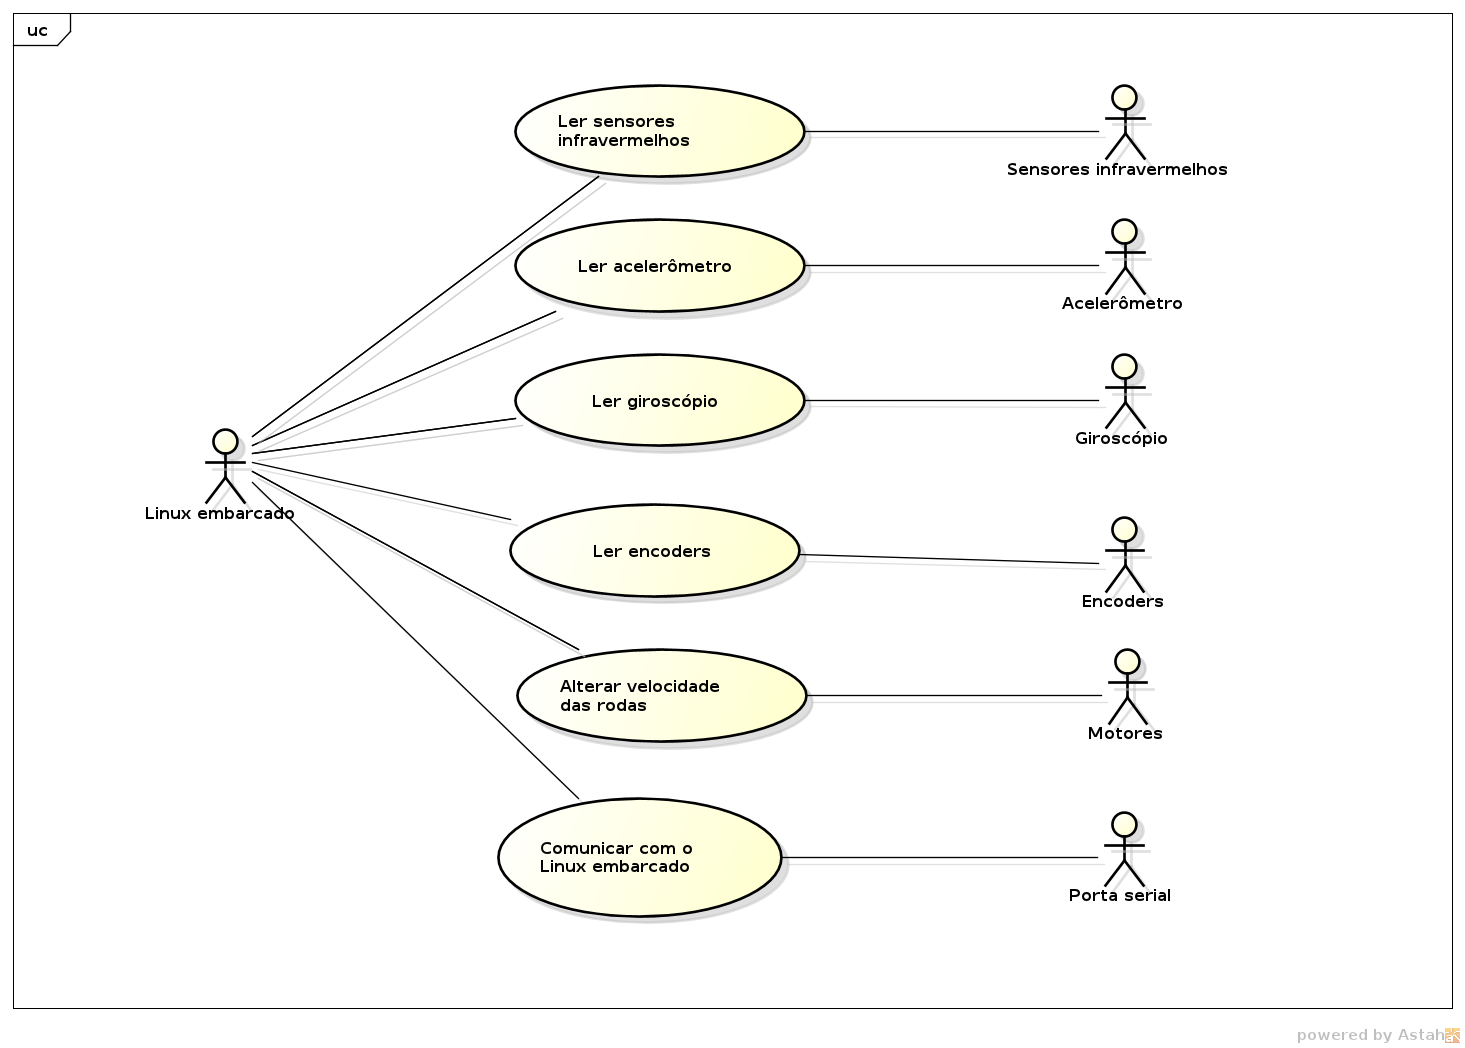
\includegraphics[width=\textwidth, keepaspectratio]{./figuras/diagrama_caso_uso_placa_embarcada.png}
  \caption{Diagrama de casos de uso do \textit{software} para a placa de baixo nível.}
  \label{fig:diagrama_caso_uso_placa_embarcada}
\end{figure}

\section{Diagrama de classes da estação base}

A Figura \ref{fig:diagrama_classes_estacao_base} mostra o diagrama de classes da estação base.
\begin{figure}[H]
  \centering
  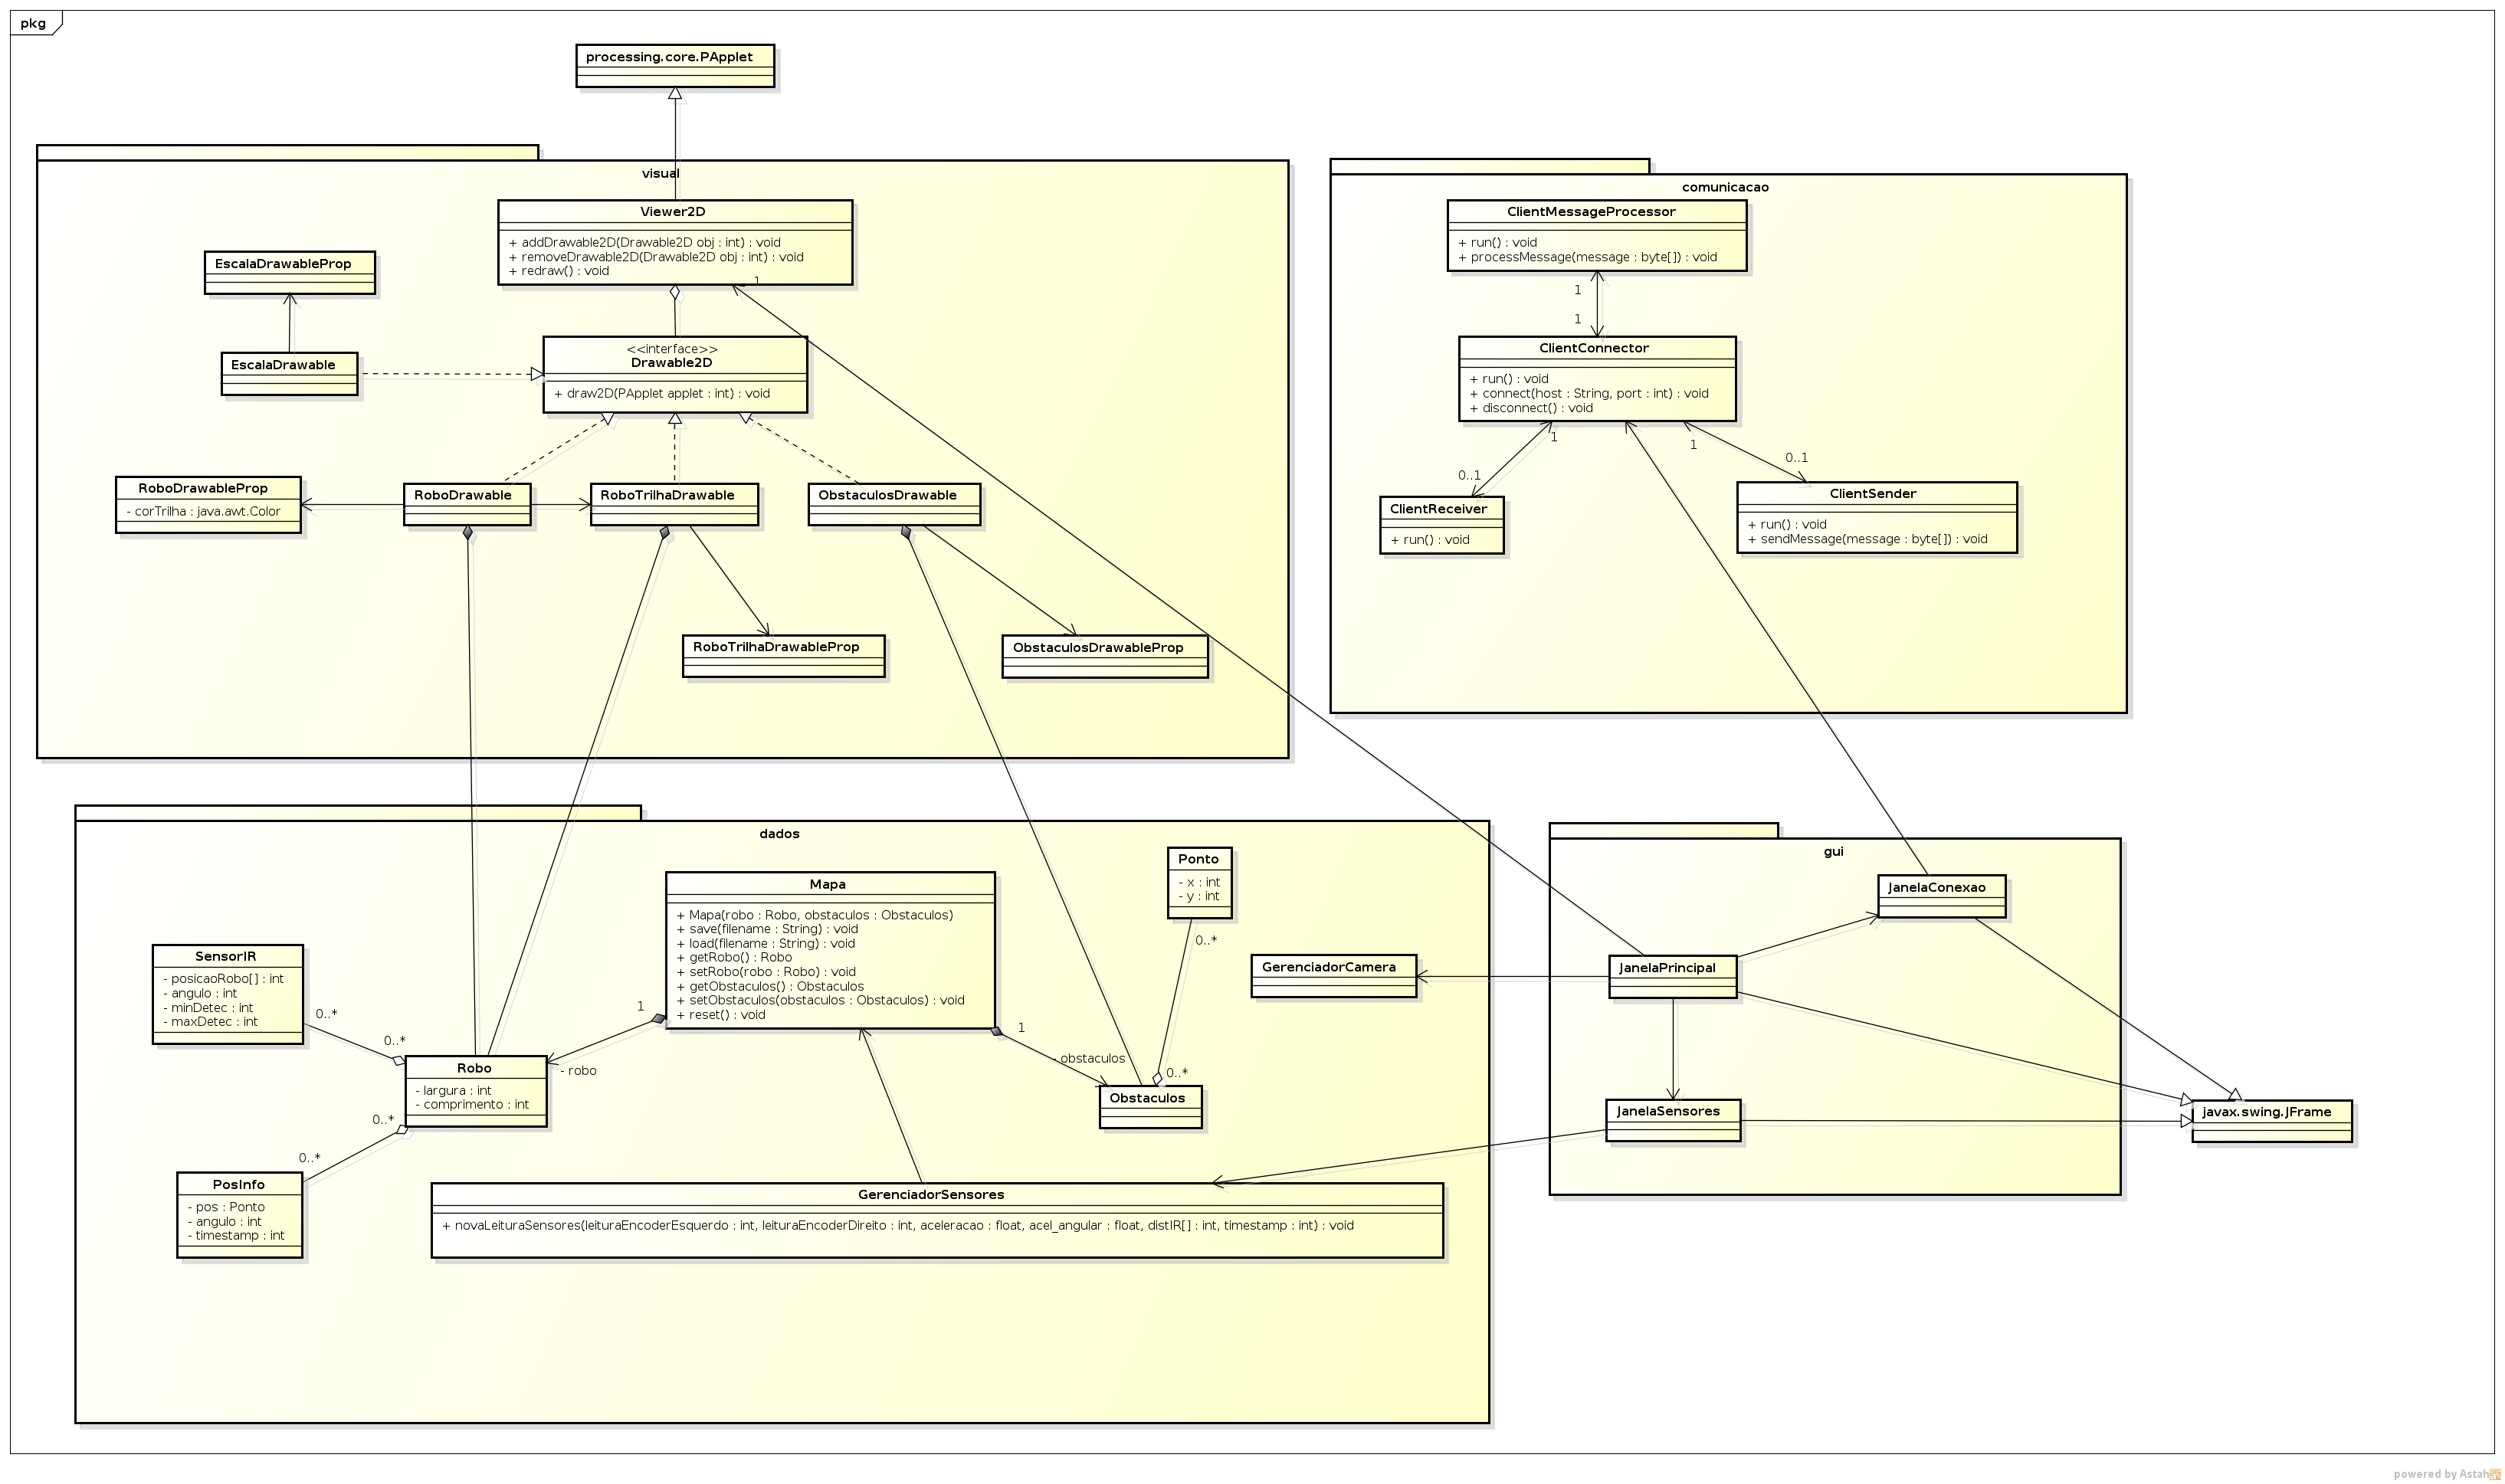
\includegraphics[width=\textwidth]{./figuras/diagrama_classes_estacao_base.png}
  \caption{Diagrama de classes da estação base}
  \label{fig:diagrama_classes_estacao_base}
\end{figure}

\subsection{Descrição das classes da estação base}
%O software da estação base do robô foi dividido em cinco pacotes:  visual, controle, comunicação, controle.robo e interface gráfica. Estes serão descritos com suas respectivas classes na Tabela \ref{tab:pacote_visual}.
O \textit{software} da estação base do robô foi dividido em cinco pacotes:  \textit{visual}, \textit{dados}, \textit{comunicao}, e \textit{gui}. A seguir há uma descrição de cada pacote e das suas respectivas classes.


\subsection{Pacote \textit{visual}}

Este pacote consiste de toda a parte visual da estação base e conta com as seguintes classes: Viewer2D, Drawable2D, EscalaDrawable, RoboDrawable, RoboTrilhaDrawable, ObstaculosDrawable, EscalaDrawableProp, RoboDrawableProp, RoboTrilhaDrawableProp e ObstaculosDrawableProp. Na Tabela \ref{tab:pacote_visual} estão descritas as classes deste pacote.


\begin{table}[h]
  \centering
  \caption{Pacote \textit{visual}}
  \begin{tabular}{p{6cm}p{8cm}}
    \toprule
    \textbf{Classe} & \textbf{Descrição} \\
    \midrule
    Viewer2D & Responsável por exibir os objetos Drawable2D. Possui recursos de pan, zoom e rotate.   \\ \hline
    Drawable2D & Representa genericamente objetos 2D que podem ser desenhados em um Viewer2D. \\ \hline
    EscalaDrawable & Responsável por desenhar uma escala gráfica no mapa. \\ \hline
    RoboDrawable & Responsável por desenhar o robô no mapa. \\ \hline
    RoboTrilhaDrawable & Responsável por desenhar a trilha percorrida pelo robô no mapa. \\ \hline
    ObstaculosDrawable & Responsável por desenhar os pontos de cada obstáculo no mapa. \\ \hline
    EscalaDrawableProp & Contém as propriedades visuais de desenho da escala. \\ \hline
    RoboDrawableProp & Contém as propriedades visuais de desenho do robô \\ \hline
    RoboTrilhaDrawableProp & Contém as propriedades visuais de desenho da trilha do robô. \\ \hline
    ObstaculosDrawableProp & Contém as propriedades visuais de desenho dos obstáculos. \\
    \bottomrule
  \end{tabular}%
  \label{tab:pacote_visual}%
\end{table}%

\subsection{Pacote \textit{dados}}

Este pacote consiste de toda a parte da estação base que processa e armazena as informações essenciais do robô e do mapa. Conta com as seguintes classes: Mapa, Obstaculos, Robo, ControleSensores, Posinfo, SensorIR e Ponto. Na Tabela \ref{tab:pacote_controle} estão descritas as classes deste pacote.

\begin{table}[h]
  \centering
  \caption{Pacote \textit{dados}}
  \begin{tabular}{p{6cm}p{8cm}}
    \toprule
    \textbf{Classe} & \textbf{Descrição} \\ 
    \midrule
    Mapa  & Responsável por representar o mapa. Armazena as informações essenciais do robô e dos obstáculos detectados. \\ \hline
    Obstaculos & Responsável por conter os obstáculos detectados pelo robô. \\ \hline
    Robo  & Responsável por representar o robô, este contêm largura, comprimento e centro de movimento (ponto central entre as duas rodas). \\ \hline
    GerenciadorSensores & Responsável por atualizar a posição do robô e dos pontos que representam os obstáculos, de acordo com as leituras feitas pelos sensores. \\ \hline
    Posinfo & Responsável por conter as informações de uma posição do robô. \\ \hline
    SensorIR & Responsável por representar um sensor IR do robô. \\ \hline 
    Ponto & Representa um ponto de cordenadas cartesianas (x,y). \\ \hline
    GerenciadorCamera & Responsável por gerenciar o status da câmera e o recebimento de imagens. \\ 
    \bottomrule
  \end{tabular}%
  \label{tab:pacote_controle}%
\end{table}%

\subsection{Pacote \textit{comunicacao}}
\label{subsec:pacote_comunicacao}

%Este pacote consiste em toda a parte de comunicação da estação base com o robô e conta com as seguintes classes: ClientCommandInterpreter, ClientConnection, ClientReceiver, ClientSender, ServerCommandInterpreter, ServerListener, ServerSender, ServerReceiver e Message. Na Tabela \ref{tab:pacote_comunicacao} estão descritas as classe deste pacote.
Este pacote consiste em toda a parte de comunicação da estação base com o robô e conta com as seguintes classes: ClientMessageProcessor ClientConnection, ClientReceiver, ClientSender e Message. Na Tabela \ref{tab:pacote_comunicacao} estão descritas as classes deste pacote.

É importante ressaltar que o protocolo TCP requer obrigatoriamente a especificação de um cliente e de um servidor para estabelecimento de uma conexão. Nas implementações desse protocolo em diversas linguagens (como Java e C++) existem tipos de \textit{socket} distintos para cliente e servidor. Na criação de um \textit{socket} de servidor, há obrigatoriamente a atribuição de uma porta de escuta, na qual o servidor aguarda que um cliente efetue uma requisição de conexão. Não é possível, ao menos nas implementações atuais do TCP, estabelecer conexão entre dois \textit{sockets} de cliente ou entre dois \textit{sockets} de servidor. Como neste projeto, o robô proverá serviços à estação base (envio de imagens da câmera, envio de leituras de sensores, além de prover a posibilidade de comando dos motores) o robô foi escolhido como servidor e a estação base como cliente. Enfatiza-se que o paradigma cliente-servidor não implica de forma alguma que a comunicação seja unidirecional. Pelo contrário, o envio de pacotes 
pode ser feito bidirecionalmente após uma conexão TCP ser estabelecida, sem nenhuma restrição quanto a isso.

\begin{table}[h]
  \centering
  \caption{Pacote \textit{comunicacao}}
  \begin{tabular}{p{6cm}p{8cm}}
    \toprule
    \textbf{Classe} & \textbf{Descrição} \\ 
    \midrule
    ClientMessageProcessor & Thread responsável pelo processamento de mensagens recebidas de um host de conexão. \\ \hline
    ClientConnector & Thread responsável por efetuar a gerência da conexão do cliente (estação base) com o servidor (robô). \\ \hline
    ClientReceiver & Thread responsável por receber mensagens de um host de uma conexão. \\ \hline
    ClientSender & Thread responsável por enviar mensagens ao host de uma conexão. \\ \hline
%    ServerCommandInterpreter & Responsável pela interpretação dos comandos do servidor. Os comandos recebidos são inseridos em uma fila, de modo a serem posteriormente executados pela thread. \\ \hline
%    Server & Responsável gerenciar o servidor (robô). \\ \hline
%    ServerListener & Responsável por escutar as novas conexões de clientes. \\ \hline
%    ServerSender & Responsável por enviar mensagens ao host de uma conexão. \\ \hline
%    ServerReceiver & Responsável por receber mensagens de um host de uma conexão. \\ \hline
%     Message & Contém uma mensagem a ser enviada por um Sender. \\ 
    \bottomrule
  \end{tabular}%
  \label{tab:pacote_comunicacao}%
\end{table}%

\subsection{Pacote \textit{gui}}

Este pacote consiste em toda a interface gráfica do sistema e conta com as seguintes classes: JanelaConexao, JanelaPrincipal e JanelaSensores. Na Tabela \ref{tab:pacote_interface_grafica} estão descritas as classes deste pacote.

\begin{table}[h]
  \centering
  \caption{Pacote \textit{gui}}
  \begin{tabular}{p{6cm}p{8cm}}
    \toprule
    \textbf{Classe} & \textbf{Descrição} \\ 
    \midrule
    JanelaConexao & Janela com as informações e configurações da conexão com o Bellator. \\ \hline
    JanelaPrincipal & Janela principal da interface gráfica da estação base. \\ \hline
    JanelaSensores & Janela de configuração dos sensores. \\ 
    \bottomrule
  \end{tabular}%
  \label{tab:pacote_interface_grafica}%
\end{table}%

\section{Fluxo de dados}

A Figura \ref{fig:diagrama_fluxo_dados} mostra o diagrama de fluxo de dados.

\begin{figure}[H]
  \centering
  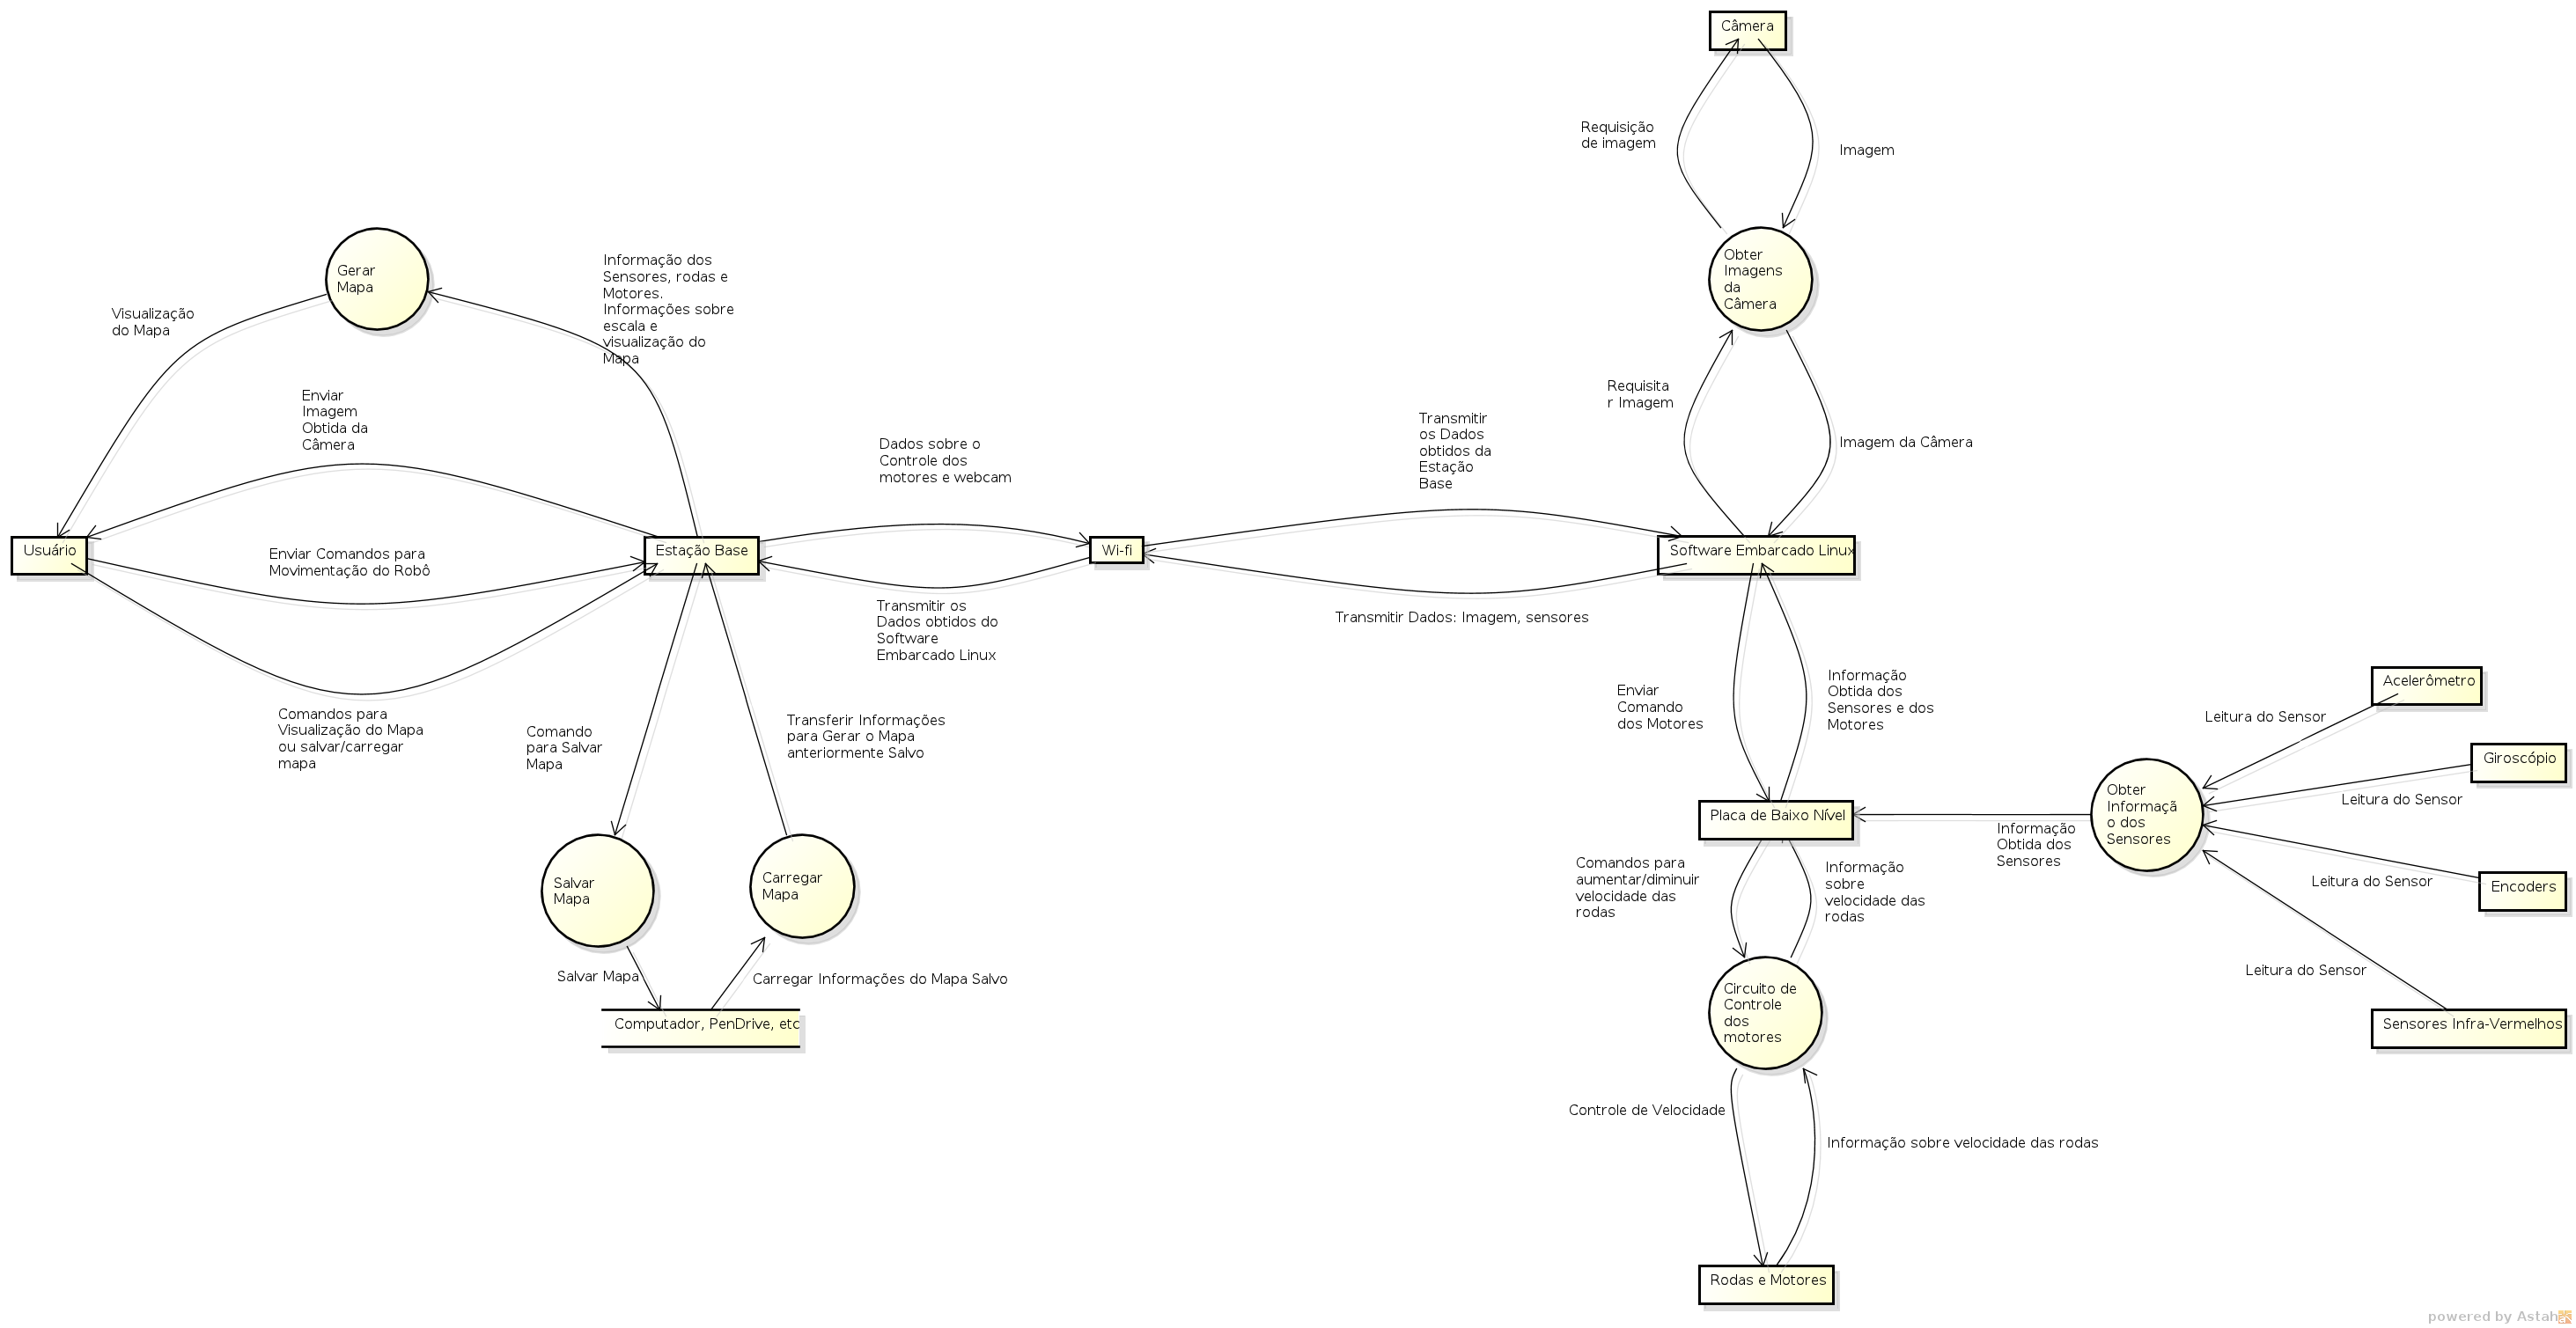
\includegraphics[width=\textwidth, keepaspectratio]{./figuras/diagrama_fluxo_dados.png}
  \caption{Diagrama de fluxo de dados.}
  \label{fig:diagrama_fluxo_dados}
\end{figure}

% \section{Diagrama de estados}
% As Figuras \ref{fig:diagrama_estados_estacao_base} e \label{fig:diagrama_estados_sistema_embarcado} mostram os diagramas de estados do sistema.
% 
% \begin{figure}[H]
%   \centering
%   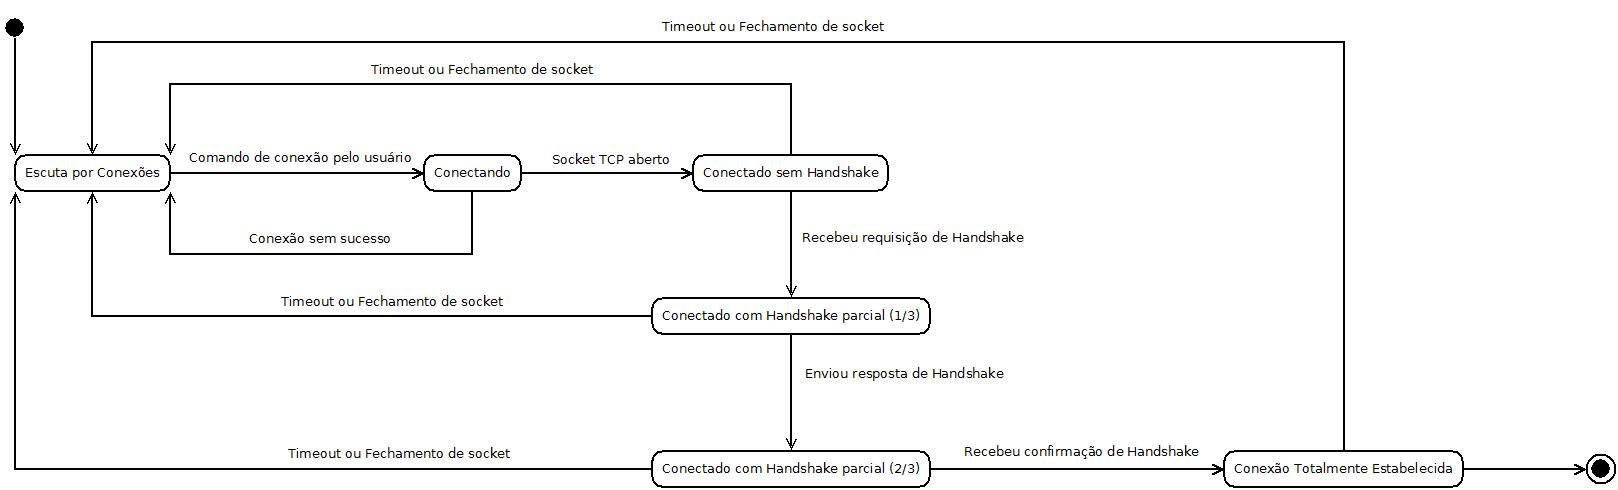
\includegraphics[width=\textwidth, keepaspectratio]{./figuras/diagrama_estados_estacao_base.jpeg}
%   \caption{Diagrama de estados para a estação base.}
%   \label{fig:diagrama_estados_estacao_base}
% \end{figure}
% 
% \begin{figure}[H]
%   \centering
%   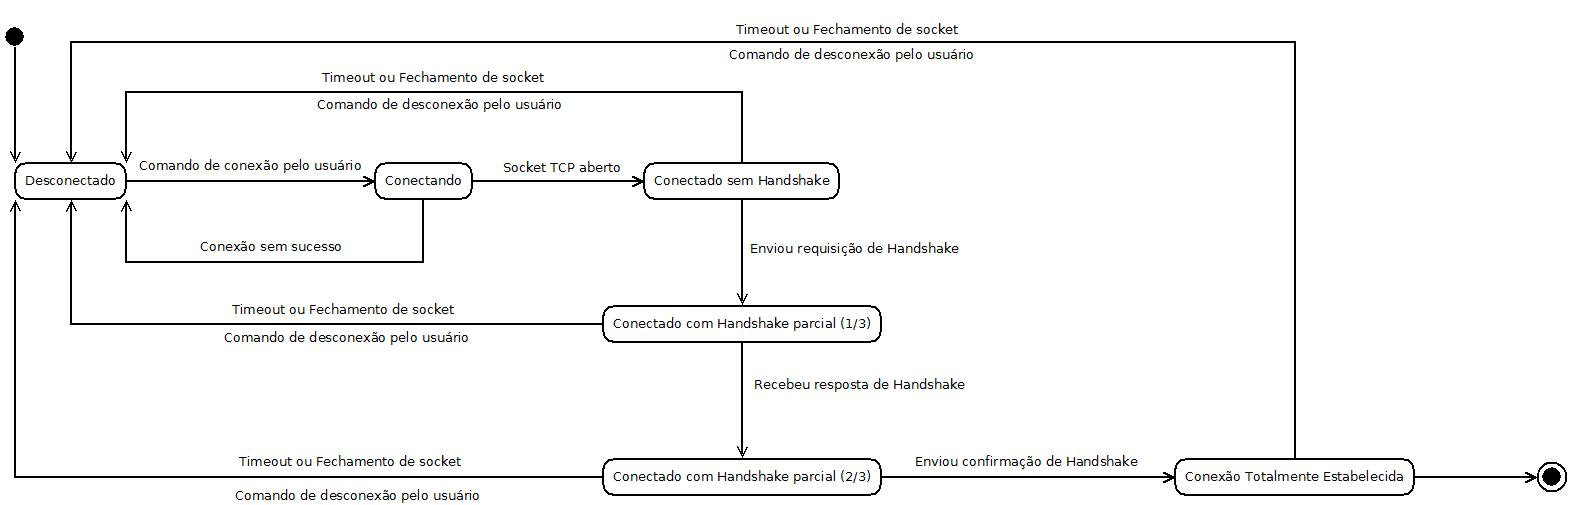
\includegraphics[width=\textwidth, keepaspectratio]{./figuras/diagrama_estados_sistema_embarcado.jpeg}
%   \caption{Diagrama de estados para o sistema embarcado.}
%   \label{fig:diagrama_estados_sistema_embarcado}
% \end{figure}


\section{Diagrama de classes do sistema embarcado}


A Figura \ref{fig:diagrama_classes_sist_embarcado} mostra o diagrama de classes do sistema embarcado (placa TS-7260).
\begin{figure}[H]
  \centering
  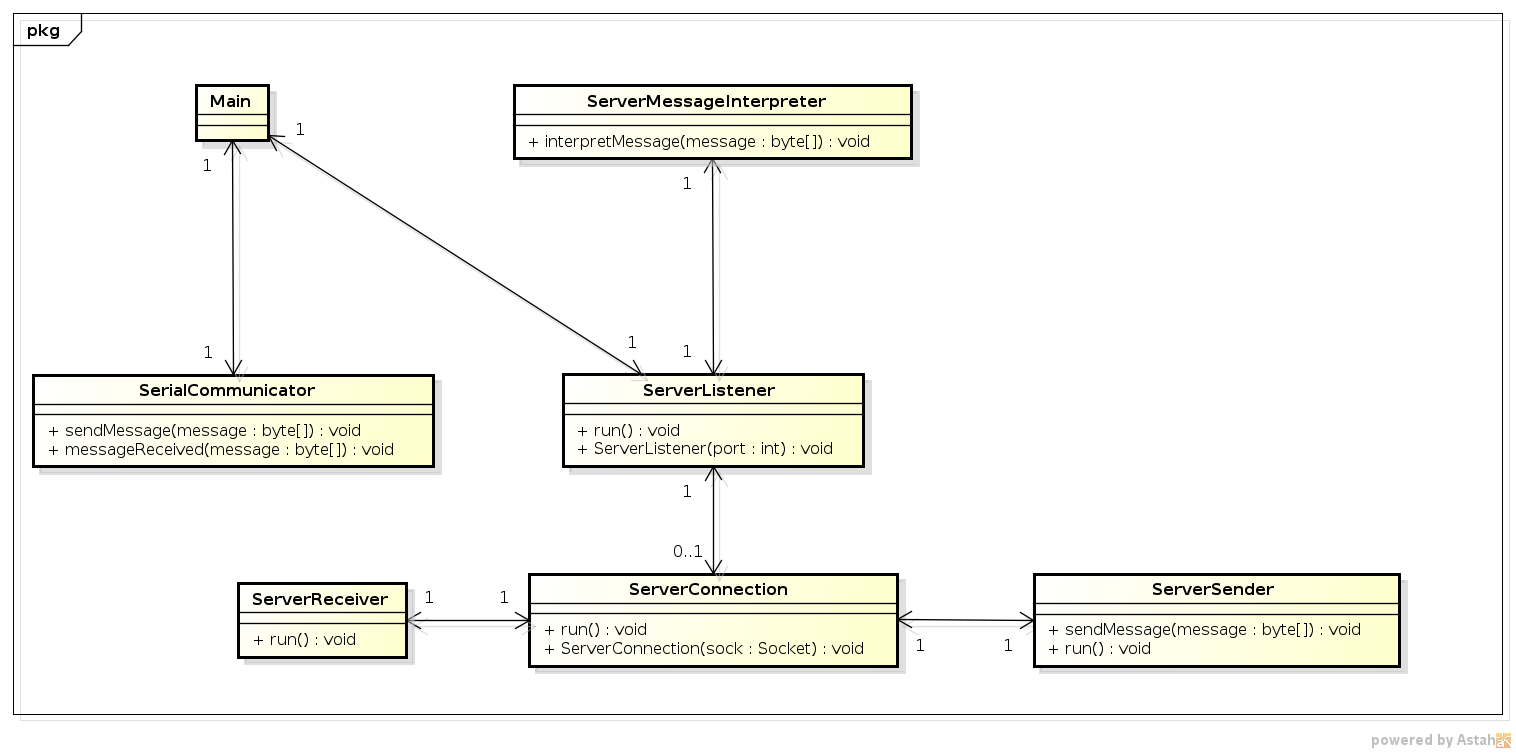
\includegraphics[width=\textwidth]{./figuras/diagrama_classes_sist_embarcado.png}
  \caption{Diagrama de classes do sistema embarcado (placa TS-7260).}
  \label{fig:diagrama_classes_sist_embarcado}
\end{figure}



%\subsection{Descrição das classes do sistema embarcado (TS-7260)}

\begin{table}[h]
  \centering
  \caption{Descrição das classes do sistema embarcado (placa TS-7260)}
  \begin{tabular}{p{6cm}p{8cm}}
    \toprule
    \textbf{Classe} & \textbf{Descrição} \\ 
    \midrule
   Main & Classe principal do robô. \\ \hline
   SensorsSampler & Thread responsável por requisitar amostras dos sensores da plca de baixo nível em intervalos de tempo previamente programados. \\ \hline
   ServerMessageProcessor & Thread responsável por realizar o processamento de mensagens recebidas de um host de conexão. \\ \hline
   ServerListener & Thread responsável por escutar requisições de conexão. \\ \hline
   ServerSender & Thread responsável por enviar mensagens ao host de uma conexão. \\ \hline
   ServerReceiver & Thread responsável por receber mensagens de um host de uma conexão. \\ \hline
   SerialCommunicator & Responsável por gerenciar a comunicação via porta serial entre a TS-7260 e a LPC2103.\\
    \bottomrule
  \end{tabular}%
  \label{tab:pacote_comunicacao}%
\end{table}%


\chapter{Diagrama de blocos do hardware}
Na figura \ref{fig:diagrama_blocos_hardware} mostra-se o diagrama de blocos do sistema embarcado e suas conexões com o restante do robô. A seguir está também uma descrição para cada um dos blocos da placa de circuito impresso do sistema embarcado.

\begin{figure}[H]
  \centering
  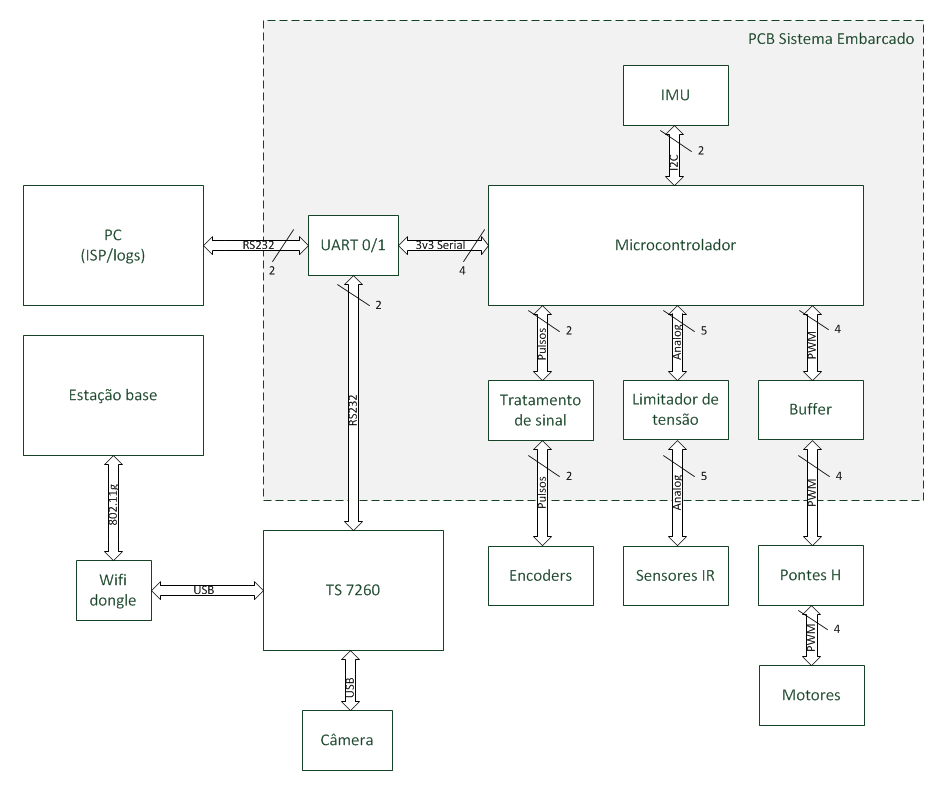
\includegraphics[width=\textwidth]{./figuras/diagrama_blocos_hardware.png}
  \caption{Diagrama de blocos do hardware}
  \label{fig:diagrama_blocos_hardware}
\end{figure}


\begin{enumerate}[topsep=0pt, partopsep=0pt, itemsep=0pt]
    \item Microcontrolador: Este bloco fará a leitura dos sensores: encoders, infra-vermelhos, acelerômetro e giroscópios. Além disso possui a implementação do protocolo de comunicação para interação com o linux embarcado da placa TS-7260.
    \item UART 0/1: Responsável por ajustar os níveis de tensão para comunicação serial no padrão RS-232 com a placa TS-7260.
    \item Buffer: Responsável por fornecer corrente e elevar os níveis de tensão de saída do microcontrolador de 3,3V para 5,0V. Esse buffer é conectado às pontes H já existentes no robô.
    \item IMU: possui o acelerômetro e o giroscópio e se comunicará com o microcontrolador por meio do protocolo I2C.
    \item Limitador de tensão: Necessário pois os sinais de saída dos sensores de infravermelho que já existem no robô não estão limitados em 5V, podendo a saída ultrapassar 5,0V e danificar o microcontrolador. 
    \item Tratamento de sinal: Composto por um filtro RC passa baixas e um schmitt trigger para remover qualquer falha que possa ocorrer na geração dos pulsos no encoder. A frequência de corte do filtro pode ser obtida pela velocidade máxima que o robô pode atingir, que foi suposta em 1 m/s (como apresentado nos requisitos de hardware).
\end{enumerate}





\raggedright
%\bibliography{referencias}

\end{document}

